\documentclass{article}
\usepackage[utf8]{inputenc}
\usepackage{parskip}
\usepackage{graphicx}
% image path
\graphicspath{{./images/}}


\title{Documento di specifica software per il progetto di Ingegneria del Software Avanzata\par
    \textit{Progetto:} \textbf{Sparql Endpoint Availability}\\}

\author{Luigi Lotito}
\date{}

\begin{document}

\maketitle
\clearpage

\tableofcontents
\clearpage

\section{Introduzione}
\label{sec:introduzione}

In questo documento si riportano le specifiche software di un servizio web che permetta
di monitorare la disponibilità degli SPARQL Endpoint, offrendo un'interfaccia web e un API REST.

Gli SPARQL endpoint, elemento fondamentale in ambito web semantico, rappresentano
un punto d'accesso per accedere  alle risorse contenute in particolari database dette basi di conoscenza (knowledge base).
I servizi che offrono SPARQL endpoint attualmente sono diverse centinaia, ma non sempre risultano attivi.
Nasce quindi la necessità di avere un punto di riferimento dove poter visualizzare
quali servizi offrono basi di conoscenza con degli SPARQL endpoint, e quali di questi sono disponibili.


\section{Requisiti}
\label{sec:requisiti}

\subsection{Sparql Endpoint Management}

In primis, il compito dell'applicazione è quello di storicizzare degli SPARQL endpoint, di cui si vuole monitorare la disponibilità.
Di ogni SPARQL endpoint si vuole memorizzare:
\begin{itemize}
    \item l'\textbf{URL} che lo identifica univocamente
    \item il \textbf{nome} o descrizione del servizio associato all'endpoint
\end{itemize}

L'applicazione deve offrire la funzionalità a degli \textbf{utenti amministratori} di poter aggiungere, modificare o rimuovere degli endpoint
dal sistema, tramite interfaccia web, o tramite API REST con autenticazione JWT.

\subsection{Sparql Endpoint monitoring and status reporting}

Ogni ora, l'applicazione deve inviare una richiesta HTTP, contente
una semplice query SPARQL, ad ogni SPARQL endpoint memorizzato nel sistema.\\
Se l'endpoint risponde, allora si considera che sia disponibile.
Gli esiti delle richieste devono essere storicizzati, in modo da poter visualizzare
la disponibilità degli endpoint attuale e nel tempo.

Per ogni query ad uno SPARQL endpoint $s$, l'applicazione deve memorizzare:
\begin{itemize}
    \item la \textbf{data} e l'\textbf{ora} della query
    \item lo \textbf{stato} dell'endpoint $s$ (attivo se ha risposto alla query, altrimenti inattivo)
\end{itemize}

In particolare l'interfaccia web deve permettere di visualizzare
la lista degli endpoint nel sistema, dove per ogni endpoint viene visulizzata:
\begin{itemize}
    \item un'eticchetta che ne rappresenta lo stato
    \item l'uptime giornaliero
    \item l'uptime settimanale
\end{itemize}

L'eticchetta dello stato è visualizzata con un indicatore colorato e in base allo stato dell'endpoint il colore è:
\begin{itemize}
    \item \textbf{verde} se l'endpoint è attivo
    \item \textbf{giallo} se l'endpoint è inattivo da meno di 24 ore
    \item \textbf{rosso} se l'endpoint è inattivo da più di 24 ore (e meno di 7 giorni)
    \item \textbf{grigio} se l'endpoint è inattivo da più di 7 giorni
\end{itemize}

L'applicazione deve offrire inoltre delle REST API per poter ottenere:
\begin{itemize}
    \item la lista degli endpoint nel sistema con il loro stato
    \item la lista degli endpoint attivi
    \item un endpoint specifico con il suo stato (conoscendone l'URL)
\end{itemize}

\subsection{User management}

Per utilizzare l'applicazione e visualizzare lo stato degli endpoint è necessario disporre di un account utente o amminstatore.
L'interfaccia web deve permettere di registrarsi, di effettuare il login e di effettuare il logout.

Per ogni utente, l'applicazione deve memorizzare:
\begin{itemize}
    \item il \textbf{nome utente}
    \item la \textbf{password} (crittografata)
    \item il \textbf{ruolo} (utente o amministratore)
    \item il \textbf{token} di autenticazione JWT (crittografato)
\end{itemize}

Un utente amministratore può aggiungere, modificare o rimuovere degli endpoint dal sistema.
Può inoltre visualizzare la lista degli utenti registrati, disabilitare o abilitare un utente, e cancellare un utente.
Un utente normale può solo visualizzare lo stato degli endpoint.
Le stesse funzionalità (con gli stessi permessi) devono essere offerte tramite API REST.

Dalla dashboard, un utente può visualizzare le informazioni relative al suo account, tra il cui token JWT utilizzabile per le API REST.

\clearpage
\section{Data flow diagram}
\label{sec:data-flow-diagram}

\begin{figure}[h]
    \centering
    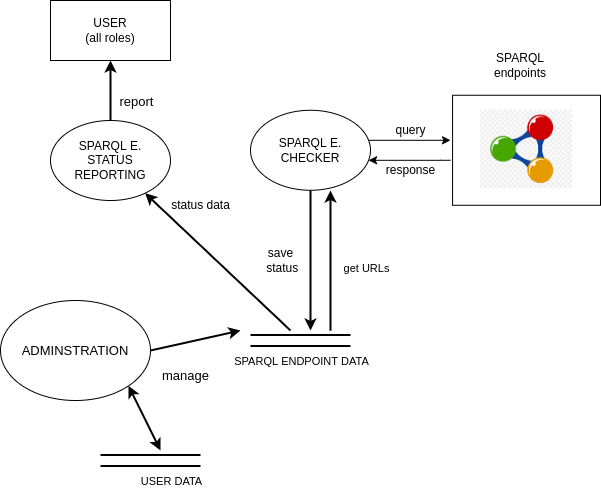
\includegraphics[width=1\textwidth]{dfd_sparql.png}
    \caption{Data flow diagram iniziale}
\end{figure}

%raffinameto di administration
\begin{figure}[h]
    \centering
    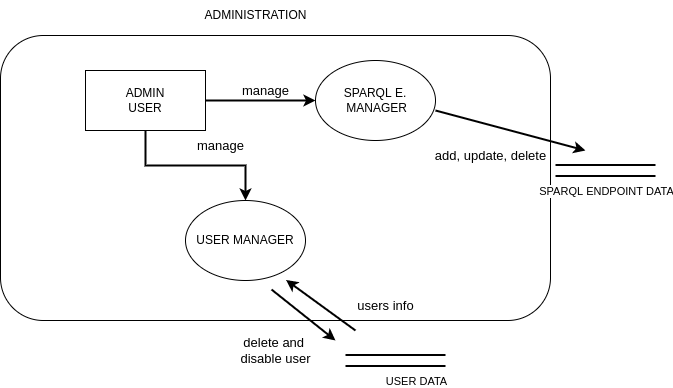
\includegraphics[width=1\textwidth]{dfd2.png}
    \caption{raffinameto di Administration}
\end{figure}

%raffinameto di sparql endpoint status reporting
\begin{figure}[h]
    \centering
    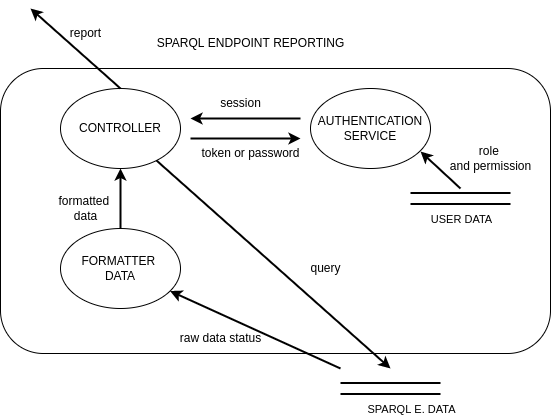
\includegraphics[width=1\textwidth]{dfd3.png}
    \caption{raffinameto di Sparql Endpoint Status Reporting}
\end{figure}

\end{document}


